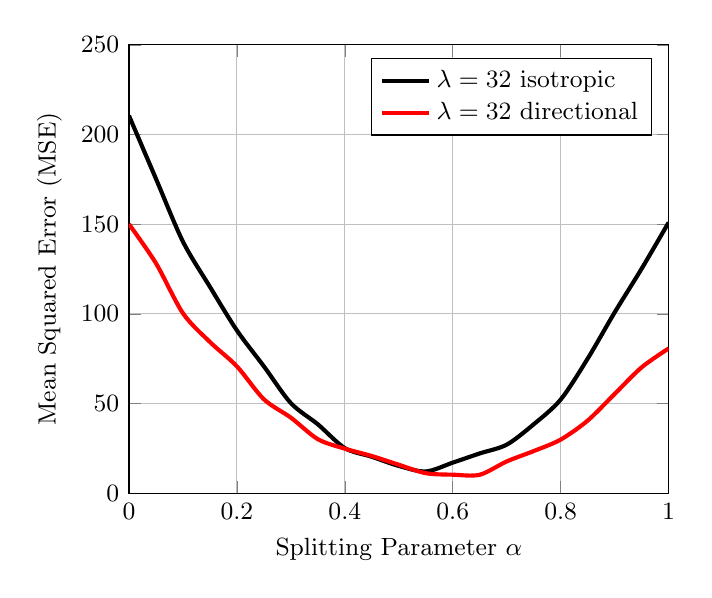
\begin{tikzpicture}
\begin{axis}[
font=\small,
xlabel= {Splitting Parameter $\alpha$},
ylabel= {Mean Squared Error (MSE)},
xmin = 0, xmax = 1,
ymin = 0, ymax = 250,
xmajorgrids,
ymajorgrids,
legend entries={$\lambda=32$ isotropic,$\lambda=32$ directional},
legend style={legend pos=north east,nodes=right}]

% Method: Bayes,
% Area Type = inscribed,
% Antenna Type = omnidirectional,
% Noise = 2,
% Trials = 50000,
% Total rate = 16,
% alpha_step =0.025,
% A_t =36.0,
% A_o =64.0,
% BMSE

\addplot [
color=black,
line width=1.5pt,
solid,smooth,
]
coordinates{
(0.0, 210.522)
(0.05, 175.363)
(0.1, 140.311)
(0.15, 115.097)
(0.2, 90.786)
(0.25, 70.768)
(0.3, 50.245)
(0.35, 38.432)
(0.4, 25.156)
(0.45, 20.332)
(0.5, 15.221)
(0.55, 12.140)
(0.6, 17.065)
(0.65, 22.211)
(0.7, 27.097)
(0.75, 38.456)
(0.8, 52.245)
(0.85, 75.064)
(0.9, 100.852)
(0.95, 125.219)
(1.0, 150.987)
};

% Method: Bayes,
% Area Type = inscribed,
% Antenna Type = directional,
% Noise = 2,
% Trials = 50000,
% Total rate = 16,
% alpha_step =0.025,
% A_t =36.0,
% A_o =64.0,
% BMSE


\addplot [
color=red,
line width=1.5pt,
solid,smooth,
]
coordinates{
	(0.0, 150.052)
	(0.05, 128.233)
	(0.1, 100.365)
	(0.15, 84.347)
	(0.2, 70.752)
	(0.25, 52.396)
	(0.3, 42.156)
	(0.35, 30.147)
	(0.4, 24.852)
	(0.45, 20.756)
	(0.5, 15.879)
	(0.55, 11.169)
	(0.6, 10.344)
	(0.65, 10.314)
	(0.7, 17.741)
	(0.75, 23.521)
	(0.8, 29.921)
	(0.85, 40.529)
	(0.9, 55.364)
	(0.95, 70.213)
	(1.0, 80.741)
};

\end{axis}

\end{tikzpicture}

